\documentclass[conference]{IEEEtran}
\IEEEoverridecommandlockouts

% Codificacao e idioma (Portugues Brasileiro)
\usepackage[utf8]{inputenc}
\usepackage[T1]{fontenc}
\usepackage[brazil]{babel}

% Pacotes padrao IEEE e matematicos
\usepackage{cite}
\usepackage{amsmath,amssymb,amsfonts}
\usepackage{algorithmic}
\usepackage{graphicx}
\usepackage{textcomp}
\usepackage{xcolor}
\usepackage{booktabs}
\usepackage{microtype}
\usepackage{url}
\usepackage{tikz}
\usetikzlibrary{arrows.meta,positioning,fit,backgrounds}

% Diretorio padrao de figuras
\graphicspath{{figuras/}}

% Rotulos em portugues para resumo e palavras-chave (opcional)
% \renewcommand{\abstractname}{Resumo}
% \renewcommand{\IEEEkeywordsname}{Palavras-chave}

\begin{document}

% TODO: Ajustar o titulo definitivo do artigo
\title{Avaliação Comparativa entre Campos Potenciais Artificiais e Algoritmo Bug2 com Odometria RK2 em Robô Móvel Diferencial}

\author{\IEEEauthorblockN{Pedro Hugo Passos da Silva Carlos}
\IEEEauthorblockA{\textit{Departamento de Engenharia Elétrica e de Computação} \\
\textit{Programa de Pós-Graduação em Engenharia Elétrica e Computação (PPGEEC)} \\
\textit{Universidade Federal da Bahia (UFBA)} \\
Salvador, Bahia, Brasil \\
pedrohugo.psc@gmail.com}
}

\maketitle

\begin{abstract}
% TODO: Redigir o resumo final apos concluir todas as secoes (nao usar simbolos matematicos, citacoes ou notas de rodape no abstract).
% Pontos sugeridos:
% - Contexto: navegacao reativa sem mapa global previo usando apenas odometria incremental e LiDAR 2D.
% - Metodologia: modelagem cinematica diferencial com integracao RK2 (Etapa I) e comparacao APF vs. Bug2 em Gazebo Harmonic + ROS 2 Jazzy (Etapa II).
% - Cenarios e protocolo: N = 5 sementes (42..46) com ruido gaussiano controlado nos cenarios A (esparsos/corredor), B (armadilha em "U") e subcenario GNRON, alem de estudo parametrico do APF.
% - Principais achados quantitativos (RMSE da odometria, taxa de sucesso, comprimento, tempo, d_min, minimos locais e GNRON).
\end{abstract}

\begin{IEEEkeywords}
Robótica Móvel, Odometria, Runge-Kutta de 2ª Ordem, Navegação Reativa, Campos Potenciais Artificiais, Algoritmo Bug2, ROS 2, Gazebo.
\end{IEEEkeywords}

% Secoes do artigo (edite cada arquivo dentro da pasta secoes/)
% Estrutura alinhada a Secao 6 (Entregaveis, item 4) do Edital PPGEE0060 2026/2
\section{Introdução}

Inicialmente, os robôs utilizavam sistemas de controle de alto nível para
evitar colisões; porém, essa abordagem nem sempre é prática quando o robô
precisa reagir rapidamente durante o deslocamento. Por conta disso,      
surgiu, na década de 1980, o controle de baixo nível, que permitiu aos   
robôs realizar o desvio de obstáculos em tempo real~\cite{khatib1986}.   
Esse método possibilitou que o robô interagisse com o ambiente de forma  
mais rápida por meio de sensores acoplados, permitindo atualmente que    
robôs aspiradores mais simples limpem o ambiente de forma autônoma sem   
utilizar um mapa~\cite{corke2023}. Por outro lado, o planejamento de     
caminho baseado em mapa (\textit{path planning}) exige construir ou      
conhecer o mapa do ambiente e saber a posição do robô em relação a ele em
todos os momentos, sendo mais comum em carros autônomos, aeronaves, entre
outros, por suportar tarefas mais complexas~\cite{corke2023}. Já para o  
exemplo do robô aspirador, a abordagem reativa torna-se adequada, pois   
sistemas reativos costumam ser mais rápidos e simples~\cite{corke2023}.  

Mesmo sem mapa global, um robô diferencial precisa manter uma estimativa 
contínua da própria pose com base na velocidade, direção e intervalo de  
deslocamento a partir de uma estimativa anterior~\cite{corke2023}.       
Existem vários métodos para realizar esse cálculo da odometria, sendo um 
deles o método de Runge-Kutta de 2ª~ordem (RK2). Para auxiliar o robô    
durante a navegação, utilizam-se sensores como os \textit{encoders} nas  
rodas (para a odometria) e o LiDAR (para a percepção local dos           
obstáculos); todavia, esses sensores não são perfeitos e acumulam        
erros~\cite{siegwart2004,corke2023}. Nesse contexto, empregam-se         
algoritmos reativos como os Campos Potenciais Artificiais
(APF)~\cite{khatib1986} e o algoritmo Bug2~\cite{lumelsky1987}, que, a   
partir da odometria estimada e das leituras locais, conduzem o robô até a
meta desviando de obstáculos.

Diante disso, o presente trabalho tem como objetivo avaliar
comparativamente os algoritmos clássicos APF e Bug2, utilizando a        
odometria calculada via RK2, em três cenários: o primeiro com obstáculos 
esparsos e um corredor até o ponto final (Cenário~A); o segundo com um   
obstáculo côncavo em formato de ``U'' antes do ponto final (Cenário~B); e
o terceiro com uma barreira posicionada atrás do ponto final (subcenário 
GNRON). Além disso, avalia-se a sensibilidade dos parâmetros do APF e    
valida-se o estimador odométrico RK2 frente ao \textit{ground truth}.

O restante deste artigo está organizado da seguinte forma: a Seção~II  
apresenta a fundamentação teórica e os trabalhos relacionados; a     
Seção~III descreve a metodologia experimental; a Seção~IV detalha o     
desenvolvimento e a implementação; a Seção~V apresenta os resultados
experimentais; a Seção~VI traz a discussão técnica e as limitações; e a 
Seção~VII apresenta as conclusões. 

\section{Fundamentação Teórica e Trabalhos Relacionados}

\subsection{Cinemática Diferencial e Odometria (RK2)}

A fim de modelar a cinemática de um robô móvel, o processo ocorre de
baixo para cima (\textit{bottom-up}), pois cada roda contribui         
individualmente para o movimento e também impõe restrições ao    
deslocamento do chassi~\cite{siegwart2004}. Desse modo, as forças e      
restrições de cada roda devem ser expressas em relação a um referencial  
consistente, tornando essencial o mapeamento entre o referencial global  
$\{X_I, Y_I\}$ e o referencial local $\{X_R, Y_R\}$, fixado no ponto     
médio $P$ do eixo motriz~\cite{siegwart2004}. Considerando a pose planar
$\boldsymbol{\xi}_I = [x,\, y,\, \theta]^T$, o mapeamento do movimento do
referencial global para o referencial local é dado
por~\cite{siegwart2004}:
\begin{equation}
\dot{\boldsymbol{\xi}}_R = R(\theta)\,\dot{\boldsymbol{\xi}}_I, 
\qquad
R(\theta) =
\begin{bmatrix}
\cos\theta & \sin\theta & 0 \\
-\sin\theta & \cos\theta & 0 \\ 
0 & 0 & 1 
\end{bmatrix}, 
\label{eq:rotacao_global_local}
\end{equation} 
em que $R(\theta)$ é a matriz de rotação ortogonal, $\theta$ representa a
orientação do robô no plano e $\dot{\boldsymbol{\xi}}$ representa o vetor
de velocidades (derivada da pose). Para mapear as velocidades do 
referencial local para o referencial global, utiliza-se a matriz inversa 
de $R(\theta)$: $\dot{\boldsymbol{\xi}}_I =
R(\theta)^{-1}\dot{\boldsymbol{\xi}}_R =
R(\theta)^T\dot{\boldsymbol{\xi}}_R$~\cite{siegwart2004}. Como nenhuma 
das rodas permite deslocamento lateral sem escorregamento, a velocidade 
lateral local é nula ($\dot{y}_R = 0$), restando apenas a velocidade 
longitudinal $\dot{x}_R = v$ e a velocidade angular $\dot{\theta}_R =
\omega$. Considerando o raio das rodas $R$ e a bitola $L = 2l$ entre     
elas, a cinemática direta a partir das velocidades angulares das rodas
direita ($\omega_d$) e esquerda ($\omega_e$) é dada 
por~\cite{siegwart2004}: 
\begin{equation}
v = \frac{R}{2}(\omega_d + \omega_e), \qquad 
\omega = \frac{R}{L}(\omega_d - \omega_e),
\label{eq:cinematica_direta} 
\end{equation}
resultando no referencial global em $\dot{x} = v\cos\theta$, $\dot{y} =
v\sin\theta$ e $\dot{\theta} = \omega$.

Conforme o robô se movimenta no ambiente, erros sistemáticos e aleatórios
nos \textit{encoders} e no contato com o solo fazem a odometria acumular 
erro de posição e, principalmente, deriva angular entre o referencial 
estimado e o original~\cite{siegwart2004,corke2023}. Na integração 
numérica discreta ao longo de um intervalo $\Delta t$, sendo $\Delta s_k 
= v_k\,\Delta t$ e $\Delta\theta_k = \omega_k\,\Delta t$, o método
clássico de Runge-Kutta de 2ª~ordem (RK2, ou Método do Ponto Médio) reduz
o erro de truncamento em curvas em comparação ao método de Euler        
explícito. Enquanto o método de Euler assume que o robô percorre toda a
distância $\Delta s_k$ mantendo a orientação inicial $\theta_k$ e gira
apenas ao final do passo~\cite{corke2023}, o RK2 considera que a       
orientação varia gradualmente de $\theta_k$ até $\theta_k +     
\Delta\theta_k$ durante $\Delta t$, adotando a direção média $\theta_k +
\Delta\theta_k/2$~\cite{siegwart2004}:
\begin{align}
x_{k+1} &= x_k + \Delta s_k \cos\!\left(\theta_k +
\frac{\Delta\theta_k}{2}\right), \label{eq:rk2_x} \\
y_{k+1} &= y_k + \Delta s_k \sin\!\left(\theta_k +
\frac{\Delta\theta_k}{2}\right), \label{eq:rk2_y} \\
\theta_{k+1} &= \operatorname{wrapToPi}(\theta_k + \Delta\theta_k),     
\label{eq:rk2_theta}
\end{align}
em que $\operatorname{wrapToPi}(\alpha) =
\operatorname{atan2}(\sin\alpha,\, \cos\alpha)$ mantém a orientação 
normalizada no intervalo $(-\pi, \pi]$.

\subsection{Campos Potenciais Artificiais (APF) e Limitações}

Para conduzir o robô até uma meta desviando de obstáculos, uma abordagem
clássica é o método dos Campos Potenciais Artificiais
(APF)~\cite{khatib1986,siegwart2004}. Nessa formulação, o robô move-se 
sob a influência de um campo potencial artificial $U(\mathbf{q})$, no 
qual a meta exerce atração e os obstáculos exercem
repulsão~\cite{siegwart2004}: 
\begin{align} 
U(\mathbf{q}) &= U_{\text{att}}(\mathbf{q}) + U_{\text{rep}}(\mathbf{q}),
\label{eq:apf_u_total} \\
U_{\text{att}}(\mathbf{q}) &= \frac{1}{2}\, k_{\text{att}}\,
\rho_{\text{goal}}^2(\mathbf{q}), \label{eq:apf_u_att} \\
U_{\text{rep}}(\mathbf{q}) &=
\begin{cases} 
\dfrac{1}{2}\, k_{\text{rep}} \left( \dfrac{1}{\rho(\mathbf{q})} -     
\dfrac{1}{\rho_0} \right)^2, & \text{se } \rho(\mathbf{q}) \le \rho_0, \\
0, & \text{se } \rho(\mathbf{q}) > \rho_0,
\end{cases} \label{eq:apf_u_rep} 
\end{align} 
em que $\mathbf{q} = [x, y]^T$ é a posição do robô, $U(\mathbf{q})$ é o
campo potencial resultante, $U_{\text{att}}(\mathbf{q})$ é o potencial
atrativo definido em~\eqref{eq:apf_u_att}, sendo $k_{\text{att}} > 0$
o ganho de atração e $\rho_{\text{goal}}(\mathbf{q}) = \|\mathbf{q} -  
\mathbf{q}_{\text{goal}}\|$ a distância euclidiana até a meta e    
$U_{\text{rep}}(\mathbf{q})$ é o potencial repulsivo definido            
em~\eqref{eq:apf_u_rep}, em que $k_{\text{rep}} > 0$ é o ganho de     
repulsão, $\rho(\mathbf{q})$ é a menor distância ao obstáculo e $\rho_0$
é o raio de influência repulsiva~\cite{siegwart2004}. 

Em termos de forças, o gradiente negativo do potencial fornece      
$\mathbf{F}(\mathbf{q}) = -\nabla U(\mathbf{q}) =
\mathbf{F}_{\text{att}}(\mathbf{q}) +
\mathbf{F}_{\text{rep}}(\mathbf{q})$~\cite{siegwart2004}:
\begin{align}
\mathbf{F}_{\text{att}}(\mathbf{q}) &= -k_{\text{att}}\,(\mathbf{q} -    
\mathbf{q}_{\text{goal}}), \label{eq:apf_f_att} \\
\mathbf{F}_{\text{rep}}(\mathbf{q}) &= 
\begin{cases} 
k_{\text{rep}} \left( \dfrac{1}{\rho(\mathbf{q})} - \dfrac{1}{\rho_0} 
\right) \dfrac{\mathbf{q} - \mathbf{q}_{\text{obs}}}{\rho^3(\mathbf{q})}, & \text{se } \rho(\mathbf{q})
\le \rho_0, \\
\mathbf{0}, & \text{se } \rho(\mathbf{q}) > \rho_0,
\end{cases} \label{eq:apf_f_rep}
\end{align}
em que $\mathbf{q}_{\text{obs}}$ denota o ponto mais próximo do obstáculo, considerando-se a superposição vetorial das forças repulsivas quando   
múltiplos obstáculos ou pontos detectados estão dentro do raio
$\rho_0$~\cite{khatib1986}. A magnitude e a direção de          
$\mathbf{F}(\mathbf{q})$ definem o movimento desejado do robô em direção 
à meta~\cite{siegwart2004}.

Contudo, o APF apresenta limitações inerentes, como a formação de mínimos
locais em obstáculos côncavos em formato de ``U'', nos quais as forças   
atrativa e repulsivas se anulam mutuamente, resultando em     
$\mathbf{F}(\mathbf{q}) = \mathbf{0}$ e impedindo o robô de sair da 
armadilha~\cite{khatib1986,koren1991}. Além dessa limitação, destacam-se
a dificuldade de atravessar passagens estreitas entre obstáculos 
próximos, o surgimento de oscilações em corredores e na proximidade de 
obstáculos~\cite{koren1991}, e o fenômeno GNRON (\textit{Goals
Nonreachable with Obstacles Nearby}), que ocorre quando um obstáculo está
muito próximo da meta: à medida que o robô se aproxima do alvo, a força
atrativa diminui enquanto a força repulsiva aumenta, fazendo com que a
posição da meta deixe de ser o mínimo global do potencial total e
impedindo o robô de alcançá-la~\cite{ge2000}.


\subsection{Algoritmo Bug2}

O algoritmo Bug2 é um método de navegação reativa que conduz o robô do
ponto de partida $S$ até o alvo $T$ combinando deslocamento em linha reta
com contorno de obstáculos~\cite{lumelsky1987}. Inicialmente, traça-se   
uma reta imaginária ligando $S$ a $T$, denominada linha-$m$              
(\textit{m-line})~\cite{corke2023}. O robô segue pela linha-$m$ em
direção ao alvo até encontrá-lo ou colidir virtualmente com um obstáculo,
registrando esse local como ponto de impacto $H^j$~\cite{lumelsky1987}.  
Ao detectar o obstáculo, o robô passa a contornar sua borda em uma       
direção fixa até reencontrar a linha-$m$ em um ponto $Q$ com caminho     
livre para o alvo que satisfaça a condição de progresso:                 
\begin{equation}
\|Q - T\| < \|H^j - T\|, 
\label{eq:bug2_progresso}
\end{equation}
em que $\|Q - T\|$ e $\|H^j - T\|$ representam as distâncias euclidianas
dos pontos $Q$ e $H^j$ até o alvo $T$. Quando essa condição é atendida, o
ponto $Q$ é definido como ponto de saída $L^j$ e o robô retoma o percurso
pela linha-$m$ rumo a $T$; caso o contorno complete uma volta fechada
retornando a $H^j$ sem encontrar saída válida, conclui-se que o alvo é   
inatingível~\cite{lumelsky1987}.

Sob condições ideais, o Bug2 garante convergência em tempo finito sempre
que houver caminho livre até a meta~\cite{lumelsky1987}. Contudo, em   
robôs móveis diferenciais reais ou simulados, a estratégia não considera 
restrições não-holonômicas nas mudanças de direção e apresenta
sensibilidade a ruídos dos sensores de alcance e à deriva odométrica ao 
tentar retornar com precisão à linha-$m$~\cite{siegwart2004,corke2023}.


\subsection{Trabalhos Relacionados}

Diversos estudos clássicos investigaram estratégias de navegação reativa sem mapa global prévio. Khatib~\cite{khatib1986} formulou o método dos Campos Potenciais Artificiais para desvio de obstáculos em tempo real combinando atração à meta e repulsão local, enquanto Koren e Borenstein~\cite{koren1991} analisaram suas limitações inerentes, destacando a ocorrência de mínimos locais em obstáculos côncavos, bloqueios em passagens estreitas e oscilações, ao passo que Ge e Cui~\cite{ge2000} formalizaram o problema GNRON quando há obstáculos próximos à meta. Como alternativa baseada em contorno topológico, Lumelsky e Stepanov~\cite{lumelsky1987} propuseram o algoritmo Bug2, demonstrando convergência em tempo finito mesmo diante de obstáculos desconhecidos de forma arbitrária. De modo complementar, Siegwart e Nourbakhsh~\cite{siegwart2004} e Corke~\cite{corke2023} sistematizam a modelagem cinemática diferencial, o acúmulo de erros na odometria discreta e os aspectos práticos desses métodos reativos em robôs móveis. Diferentemente de análises puramente teóricas ou com pose ideal, o presente trabalho avalia comparativamente o APF e o Bug2 sob odometria RK2 com ruído controlado, investigando o compromisso entre suavidade de trajetória e convergência em cenários com obstáculos esparsos, armadilha em ``U'' e bloqueio próximo à meta.

\section{Metodologia Experimental}

\subsection{Plataforma de Simulação e Modelo do Robô}
% TODO: Descrever o ambiente (Ubuntu 24.04, ROS 2 Jazzy Jalisco, Gazebo Sim 8.11.0 Harmonic) e a geometria calibrada do robo diferencial (base_link no centro do eixo motriz, colisoes esfericas pontuais com L_eff = 0,35 m, sensores e limites cinematicos/dinamicos).
% Referenciar a Tabela~\ref{tab:parametros}.

\begin{table}[htbp]
\centering
\caption{Parâmetros do robô diferencial, sensores e controladores avaliados.}
\label{tab:parametros}
\setlength{\tabcolsep}{3.5pt}
\resizebox{\columnwidth}{!}{%
\begin{tabular}{llc}
\toprule
\textbf{Componente} & \textbf{Parâmetro} & \textbf{Valor} \\
\midrule
Robô diferencial & Raio das rodas ($R$) & $0{,}05\text{ m}$ \\
                 & Bitola entre rodas ($L$) & $0{,}35\text{ m}$ \\
                 & Limites cinemáticos ($v_{\max}, \omega_{\max}$) & $0{,}40\text{ m/s}$, $1{,}20\text{ rad/s}$ \\
\midrule
Sensores         & Frequência dos encoders / odometria RK2 & $100\text{ Hz}$ / $50\text{ Hz}$ \\
                 & Ruído nos encoders ($\sigma_\omega$) & $0{,}05\text{ rad/s}$ \\
                 & LiDAR 2D planar ($360$ feixes, $20\text{ Hz}$) & $[0{,}12\text{ m},\, 8{,}0\text{ m}]$ \\
                 & Ruído no LiDAR ($\sigma_\rho$) & $0{,}01\text{ m}$ \\
\midrule
APF (nominal)    & Ganhos ($k_{\text{att}}, k_{\text{rep}}$) & $1{,}0$, $0{,}8$ \\
                 & Raio de influência repulsiva ($\rho_0$) & $1{,}10\text{ m}$ \\
                 & Ganhos cinemáticos ($k_v, k_\omega$) & $0{,}25$, $1{,}8$ \\
\midrule
Bug2             & Distâncias ($d_{\text{hit}}, d_{\text{wall}}, d_{\text{debounce}}$) & $0{,}52\text{ m}$, $0{,}45\text{ m}$, $0{,}45\text{ m}$ \\
                 & Tolerância à linha-$m$ ($\delta_m$) e progresso ($\epsilon$) & $0{,}10\text{ m}$, $0{,}15\text{ m}$ \\
\midrule
Protocolo        & Tolerância à meta ($d_{\text{tol}}$) & $0{,}20\text{ m}$ \\
                 & Sementes aleatórias ($N=5$) & $\{42, 43, 44, 45, 46\}$ \\
\bottomrule
\end{tabular}%
}
\end{table}


\subsection{Protocolo da Etapa I --- Validação da Odometria}
% TODO: Descrever as 3 trajetorias de teste em arena livre (mundo_etapa1_vazio.sdf):
% 1. Linha reta (5 m)
% 2. Arco circular (R_c = 1 m)
% 3. Percurso composto em "S"
% Explicar a frequencia de integracao (50 Hz), uso de use_sim_time e comparacao contra /ground_truth/odom.

\subsection{Protocolo da Etapa II --- Cenários de Navegação e Estudo Paramétrico}
% TODO: Descrever os 3 cenarios (arquivos .sdf), posicoes de partida S=(0,0) e meta T, e o estudo parametrico:
% - Cenario A (cenario_a_esparsos.sdf): obstaculos convexos esparsos + corredor, T=(8,0).
% - Cenario B (cenario_b_armadilha_u.sdf): parede concava em "U", T=(6,0).
% - Subcenario GNRON (cenario_gnron.sdf): parede a 0,45 m atras da meta T=(6,0).
% - Estudo parametrico do APF no Cenario A (Fraco, Nominal, Forte, Ganho Alto) e variacao de rho_0 no GNRON (0,35; 0,80; 1,10; 1,50 m).

\subsection{Métricas de Avaliação e Repetibilidade}
% TODO: Definir formalmente:
% - Etapa I: erros instantaneos e_p(t), e_theta(t) e RMSE_p, RMSE_theta.
% - Etapa II: Taxa de sucesso (%), Colisoes, Comprimento L_traj (m), Tempo total T_tot (s), Distancia minima aos obstaculos d_min (m), Taxa de bloqueio / minimos locais (%), Erro odométrico final e_p(t_f) e Distancia real a meta d_meta (m).
% - Repetibilidade: N = 5 sementes fixas {42, 43, 44, 45, 46} com ruido branco gaussiano nos encoders (sigma_omega = 0,05 rad/s) e no LiDAR (sigma_rho = 0,01 m).

\section{Desenvolvimento e Implementação}

\subsection{Arquitetura Modular em ROS 2 Jazzy e Gazebo Harmonic}
% TODO: Descrever os pacotes, plugins SDF do modelo robo_diferencial (diff-drive, joint-state-publisher, gpu_lidar, odometry-publisher), bridge ros_gz_bridge (bridge_params.yaml), QoS (qos_profile_sensor_data em /scan) e sincronizacao temporal (/clock).
% Referenciar a Figura~\ref{fig:arquitetura_ros2} e as referencias \cite{ros2jazzy,gazeboharmonic}.

\begin{figure}[htbp]
\centering
\resizebox{\columnwidth}{!}{\begin{tikzpicture}[
    font=\scriptsize,
    >=Stealth,
    sim/.style={
        rectangle, rounded corners=2.5pt, draw=black!80, fill=gray!12,
        thick, minimum width=3.3cm, minimum height=0.95cm, align=center, inner sep=4pt
    },
    bridge/.style={
        rectangle, rounded corners=2.5pt, draw=teal!75!black, fill=teal!10,
        thick, minimum width=3.3cm, minimum height=0.95cm, align=center, inner sep=4pt
    },
    rosnode/.style={
        rectangle, rounded corners=2.5pt, draw=blue!70!black, fill=blue!8,
        thick, minimum width=3.7cm, minimum height=0.95cm, align=center, inner sep=4pt
    },
    eval/.style={
        rectangle, rounded corners=2.5pt, draw=orange!80!black, fill=orange!10,
        thick, minimum width=3.7cm, minimum height=0.95cm, align=center, inner sep=4pt
    },
    topic/.style={
        font=\ttfamily\scriptsize, inner sep=1.5pt
    }
]

% Coluna esquerda: Simulador e Ponte
\node[sim]    (gz)     at (0, 0.3)    {\textbf{Gazebo Harmonic}\\\texttt{robo\_diferencial} (.sdf)};
\node[bridge] (br)     at (0, -1.7)   {\textbf{\texttt{ros\_gz\_bridge}}\\\texttt{/clock}, sensores e \texttt{/cmd\_vel}};

% Coluna direita: Avaliacao, Estimacao e Controle
\node[eval]    (logger) at (7.2, 0.3)  {\textbf{Nós Avaliadores}\\\texttt{metrics\_logger} / \texttt{nav\_metrics}};
\node[rosnode] (odom)   at (7.2, -1.7) {\textbf{\texttt{odom\_estimator}}\\Integração RK2 ($50\text{ Hz}$)};
\node[rosnode] (nav)    at (7.2, -3.7) {\textbf{Controlador Reativo}\\\texttt{apf\_navigator} / \texttt{bug2\_navigator}};

% 1) Gazebo <-> Bridge
\draw[<->, thick] (gz.south) -- node[right=2pt, font=\scriptsize] {Gz Transport} (br.north);

% 2) Ground Truth isolado (Bridge -> Avaliadores)
\draw[->, dashed, thick, orange!85!black]
    ([yshift=0.22cm]br.east) -- (2.05, -1.48) -- (2.05, 0.3)
    -- node[midway, above=2pt, topic, text=orange!75!black] {/ground\_truth/odom} (logger.west);

% 3) Encoders (Bridge -> Odom)
\draw[->, thick]
    ([yshift=-0.12cm]br.east) -- ([yshift=-0.12cm]odom.west)
    node[pos=0.58, below=2pt, topic] {/joint\_states};

% 4) LiDAR (Bridge -> Controlador)
\draw[->, thick]
    ([xshift=0.55cm]br.south) |- ([yshift=0.12cm]nav.west)
    node[pos=0.73, above=2pt, topic] {/scan (best\_effort)};

% 5) Odometria estimada (Odom -> Controlador e Odom -> Avaliadores)
\draw[->, thick] (odom.south) -- node[right=2pt, topic] {/odom\_est} (nav.north);
\draw[->, thick] (odom.north) -- node[right=2pt, topic] {/odom\_est} (logger.south);

% 6) Comando de velocidade (Controlador -> Bridge)
\draw[->, thick]
    (nav.south) -- ++(0, -0.55) -| ([xshift=-0.55cm]br.south)
    node[pos=0.25, below=2pt, topic] {/cmd\_vel};

% 7) Status e eventos (Controlador -> Avaliadores pela direita)
\draw[->, thick]
    (nav.east) -- ++(0.45, 0) |- (logger.east)
    node[pos=0.25, right=2pt, topic, align=left] {/nav\_status\\/nav\_events};

\end{tikzpicture}
}
\caption{Arquitetura modular em ROS~2 Jazzy e Gazebo Harmonic com isolamento estrito do tópico \texttt{/ground\_truth/odom}.}
\label{fig:arquitetura_ros2}
\end{figure}

\subsection{Estimador de Odometria (\texttt{odom\_estimator\_node})}
% TODO: Detalhar a implementacao do no odom_estimator_node.py e do modulo kinematic_model.py (leitura de /joint_states, injecao opcional de ruido gaussiano com seed fixa, passo RK2 e publicacao em /odom_est).

\subsection{Controladores Reativos: APF e Bug2}

Ambos os controladores operam em malha fechada a $20\text{ Hz}$ assinando exclusivamente \texttt{/odom\_est} e \texttt{/scan}, sem acesso ao \textit{ground truth}, e encerram a navegação com sucesso quando a distância estimada até a meta é inferior à tolerância $d_{\text{tol}}$ ($0{,}20\text{ m}$).

No nó \texttt{apf\_navigator\_node}, a força resultante é obtida somando a atração para a meta às contribuições repulsivas dos feixes do LiDAR que detectam obstáculos dentro do raio $\rho_0$. Como o robô diferencial não se desloca lateralmente, a direção e a magnitude dessa força resultante são convertidas em comandos de velocidade angular e linear por meio dos ganhos cinemáticos $k_\omega$ e $k_v$ (Tabela~\ref{tab:parametros}), reduzindo a velocidade linear quando o erro de orientação é elevado para que o robô gire antes de avançar. Quando o deslocamento do robô permanece desprezível por um intervalo contínuo, o controlador identifica automaticamente a estagnação por mínimo local ou GNRON.

No nó \texttt{bug2\_navigator\_node}, o algoritmo clássico~\cite{lumelsky1987} foi implementado como uma máquina de estados finitos alternando entre busca direta (\texttt{GOAL\_SEEKING}) e contorno de obstáculo (\texttt{WALL\_FOLLOWING}), com ajustes práticos necessários para lidar com as dimensões físicas do robô, a discretização temporal e o ruído sensorial~\cite{siegwart2004}. No modo \texttt{GOAL\_SEEKING}, o robô segue a linha-$m$ rumo à meta até detectar um obstáculo frontal dentro do limiar $d_{\text{hit}}$, registrando o ponto de impacto $H^j$ e iniciando o contorno. No modo \texttt{WALL\_FOLLOWING}, o controlador mantém o obstáculo a uma distância lateral segura $d_{\text{wall}}$ até satisfazer simultaneamente as condições práticas de saída para o ponto $L^j$: ter percorrido um trecho mínimo de contorno $d_{\text{debounce}}$ (evitando trocas falsas de estado logo após $H^j$), reencontrar a linha-$m$ dentro da faixa de tolerância $\delta_m$, estar mais próximo da meta do que $H^j$ por uma margem mínima $\epsilon$ e possuir caminho frontal livre na direção do alvo.

\subsection{Isolamento do \textit{Ground Truth} e Registro de Métricas}
% TODO: Explicar a garantia arquitetural de que apenas metrics_logger_node.py e nav_metrics_logger_node.py assinam /ground_truth/odom, alem da orquestracao automatizada das baterias (scripts run_etapa1.py e run_fase6_experimentos.py).

\section{Resultados Experimentais}

\subsection{Etapa I: Validação da Odometria RK2}
% TODO: Analisar os resultados da Tabela~\ref{tab:etapa1_odometria}, Figura~\ref{fig:etapa1_trajetorias} e Figura~\ref{fig:etapa1_erros} para as 3 trajetorias (reta, arco circular e percurso composto em "S").

\begin{table}[htbp]
\centering
\caption{Métricas de erro da odometria RK2 em relação ao \textnormal{\textit{ground truth}} na Etapa I.}
\label{tab:etapa1_odometria}
\setlength{\tabcolsep}{3.5pt}
\resizebox{\columnwidth}{!}{%
\begin{tabular}{lccccc}
\toprule
\textbf{Trajetória} & \textbf{Comp. (m)} & \textbf{$\text{RMSE}_p$ (m)} & \textbf{$e_p(t_f)$ (m)} & \textbf{$\text{RMSE}_\theta$ ($^\circ$)} & \textbf{$e_\theta(t_f)$ ($^\circ$)} \\
\midrule
Linha Reta (5 m)        & 4,99 & 0,0039 & 0,0061 & 0,05 & 0,04 \\
Arco Circular ($R_c=1$ m) & 6,26 & 0,0042 & 0,0055 & 0,23 & 0,31 \\
Percurso Composto (``S'') & 4,99 & 0,0036 & 0,0039 & 0,17 & 0,04 \\
\bottomrule
\end{tabular}%
}
\end{table}


\begin{figure*}[t]
\centering
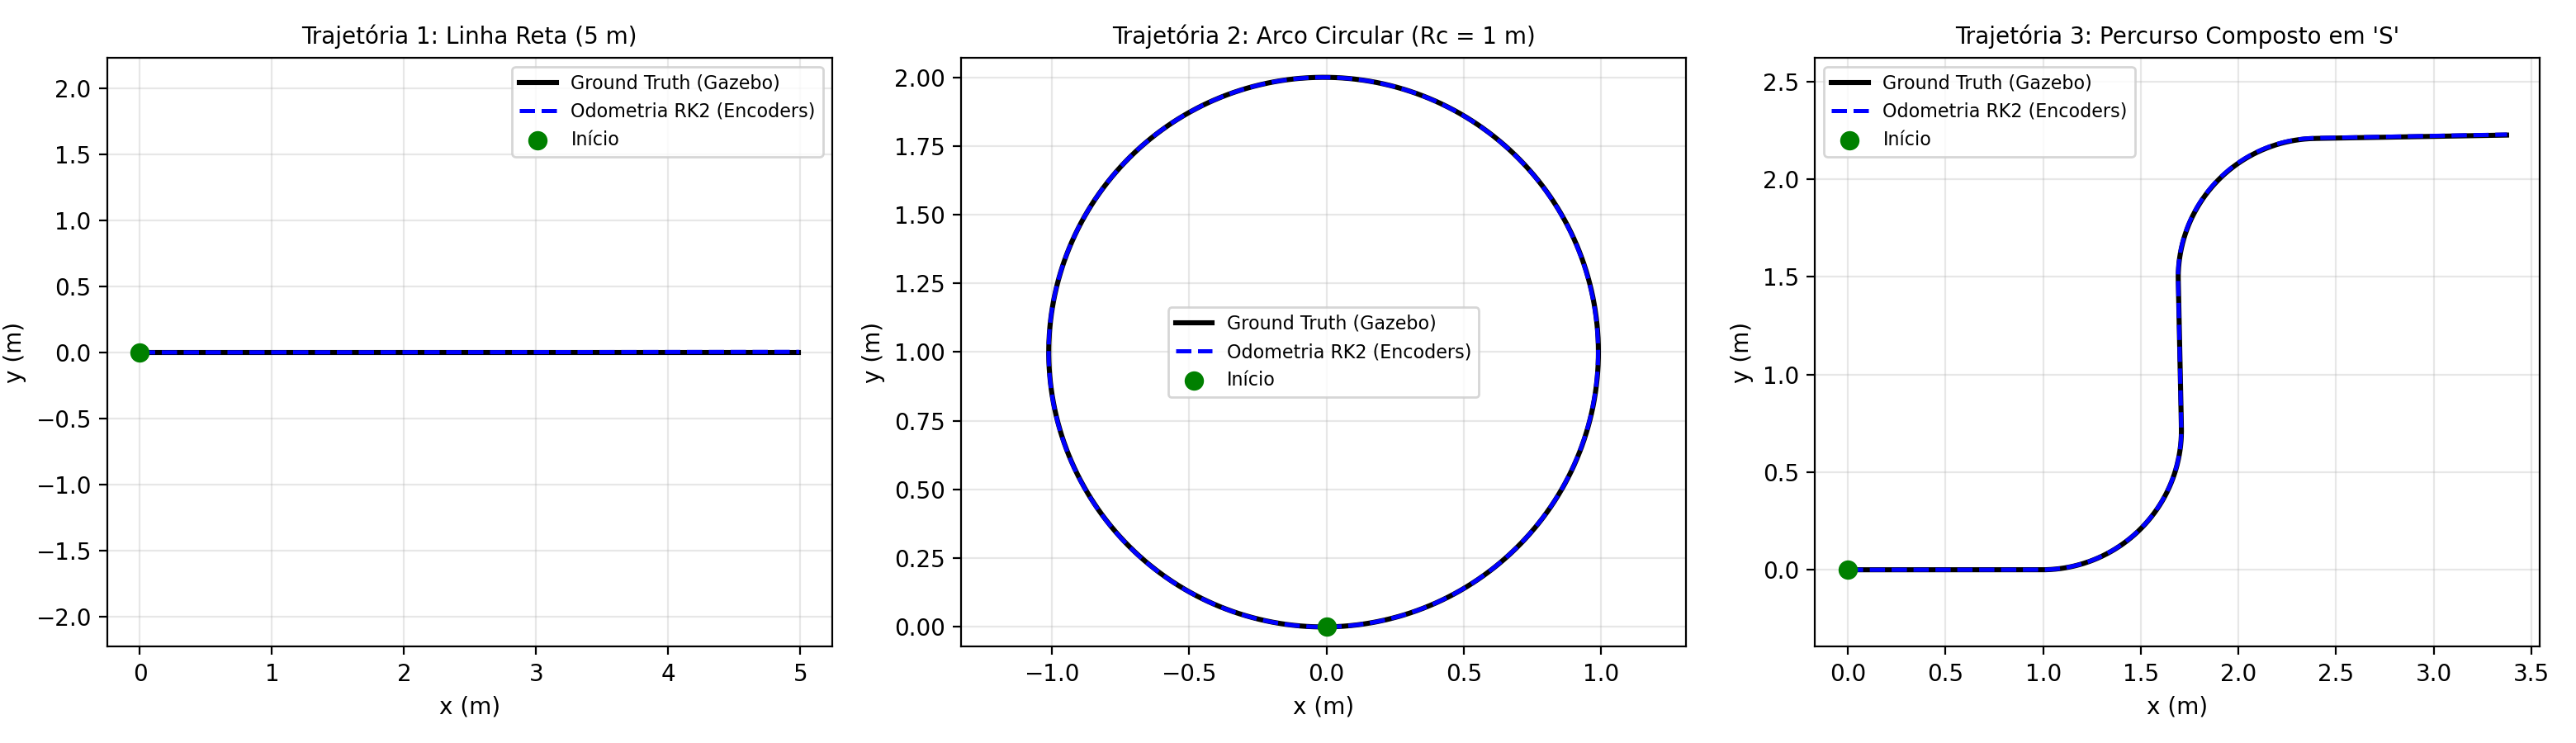
\includegraphics[width=\textwidth]{fig1_etapa1_trajetorias.png}
\caption{Comparação entre as trajetórias estimadas pela odometria RK2 e o \textit{ground truth} do simulador na Etapa~I.}
\label{fig:etapa1_trajetorias}
\end{figure*}

\begin{figure*}[t]
\centering
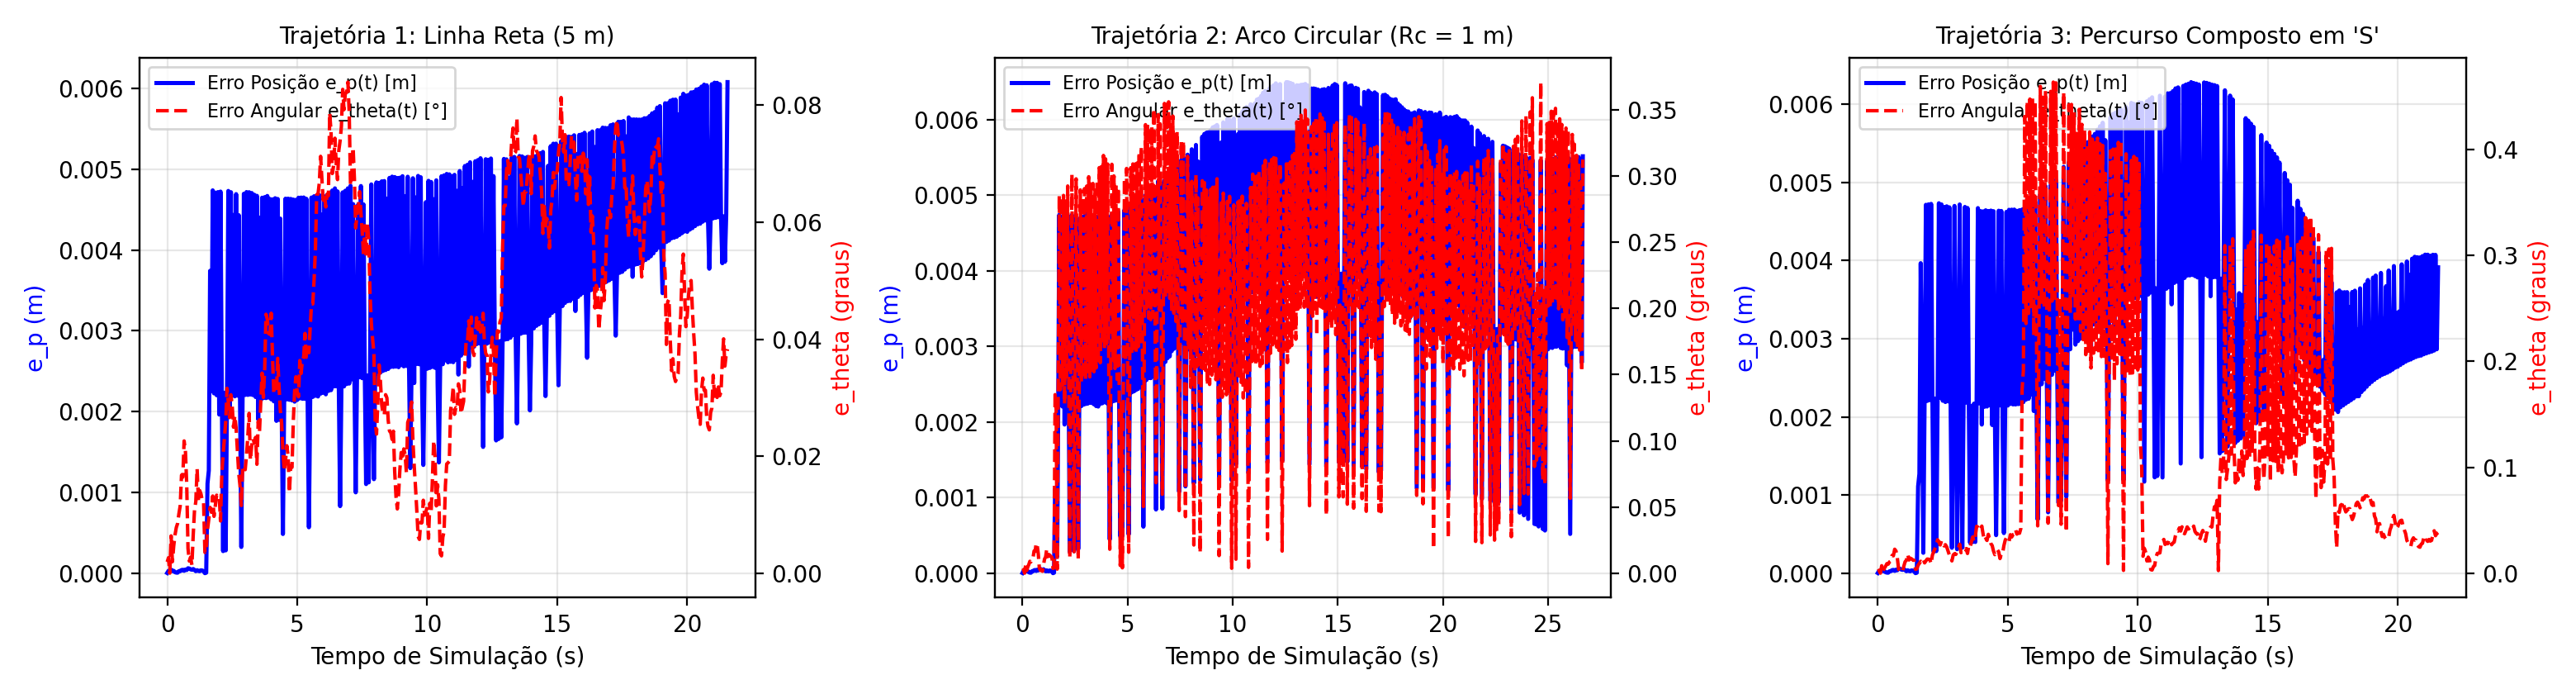
\includegraphics[width=\textwidth]{fig2_etapa1_erros.png}
\caption{Evolução temporal dos erros de posição $e_p(t)$ e orientação $e_\theta(t)$ na Etapa~I.}
\label{fig:etapa1_erros}
\end{figure*}

\subsection{Etapa II: Comparação APF vs. Bug2 nos Cenários A, B e GNRON}
% TODO: Analisar a Tabela~\ref{tab:comparacao_p6} e a Figura~\ref{fig:etapa2_cenarios} (N = 5 sementes, media +/- desvio padrao) destacando o comportamento de cada metodo nos Cenarios A, B e GNRON.

\begin{table*}[t]
\centering
\caption{Comparação quantitativa entre APF e Bug2 nos cenários experimentais ($N = 5$ execuções, sementes 42--46, média $\pm$ desvio padrão).}
\label{tab:comparacao_p6}
\setlength{\tabcolsep}{4pt}
\resizebox{\textwidth}{!}{%
\begin{tabular}{llcccccccc}
\toprule
\textbf{Cenário} & \textbf{Método} & \textbf{Sucesso (\%)} & \textbf{Colisões} & \textbf{$L_{\text{traj}}$ (m)} & \textbf{$T_{\text{tot}}$ (s)} & \textbf{$d_{\min}$ (m)} & \textbf{Bloqueios (\%)} & \textbf{$e_p(t_f)$ (m)} & \textbf{$d_{\text{meta}}$ (m)} \\
\midrule
Cenário A (Esparsos) & APF & 100\% & 0 & $10{,}01 \pm 0{,}00$ & $33{,}4 \pm 0{,}1$ & $0{,}28 \pm 0{,}00$ & 0\% & $0{,}0060 \pm 0{,}0027$ & $0{,}20 \pm 0{,}01$ \\
Cenário A (Esparsos) & Bug2 & 100\% & 0 & $9{,}68 \pm 0{,}02$ & $37{,}2 \pm 0{,}2$ & $0{,}36 \pm 0{,}00$ & 0\% & $0{,}0098 \pm 0{,}0033$ & $0{,}20 \pm 0{,}01$ \\
\midrule
Cenário B (Armadilha ``U'') & APF & 0\% & 0 & $3{,}05 \pm 0{,}00$ & $13{,}2 \pm 0{,}0$ & $0{,}47 \pm 0{,}00$ & 100\% & $0{,}0005 \pm 0{,}0006$ & $3{,}14 \pm 0{,}00$ \\
Cenário B (Armadilha ``U'') & Bug2 & 100\% & 0 & $12{,}25 \pm 0{,}02$ & $45{,}9 \pm 0{,}1$ & $0{,}38 \pm 0{,}00$ & 0\% & $0{,}0096 \pm 0{,}0022$ & $0{,}20 \pm 0{,}01$ \\
\midrule
Cenário GNRON & APF & 0\% & 0 & $5{,}65 \pm 0{,}00$ & $22{,}6 \pm 0{,}0$ & $0{,}80 \pm 0{,}00$ & 100\% & $0{,}0018 \pm 0{,}0012$ & $0{,}35 \pm 0{,}00$ \\
Cenário GNRON & Bug2 & 100\% & 0 & $5{,}81 \pm 0{,}00$ & $17{,}2 \pm 0{,}0$ & $0{,}66 \pm 0{,}00$ & 0\% & $0{,}0039 \pm 0{,}0007$ & $0{,}19 \pm 0{,}00$ \\
\bottomrule
\end{tabular}%
}
\end{table*}


\begin{figure*}[t]
\centering
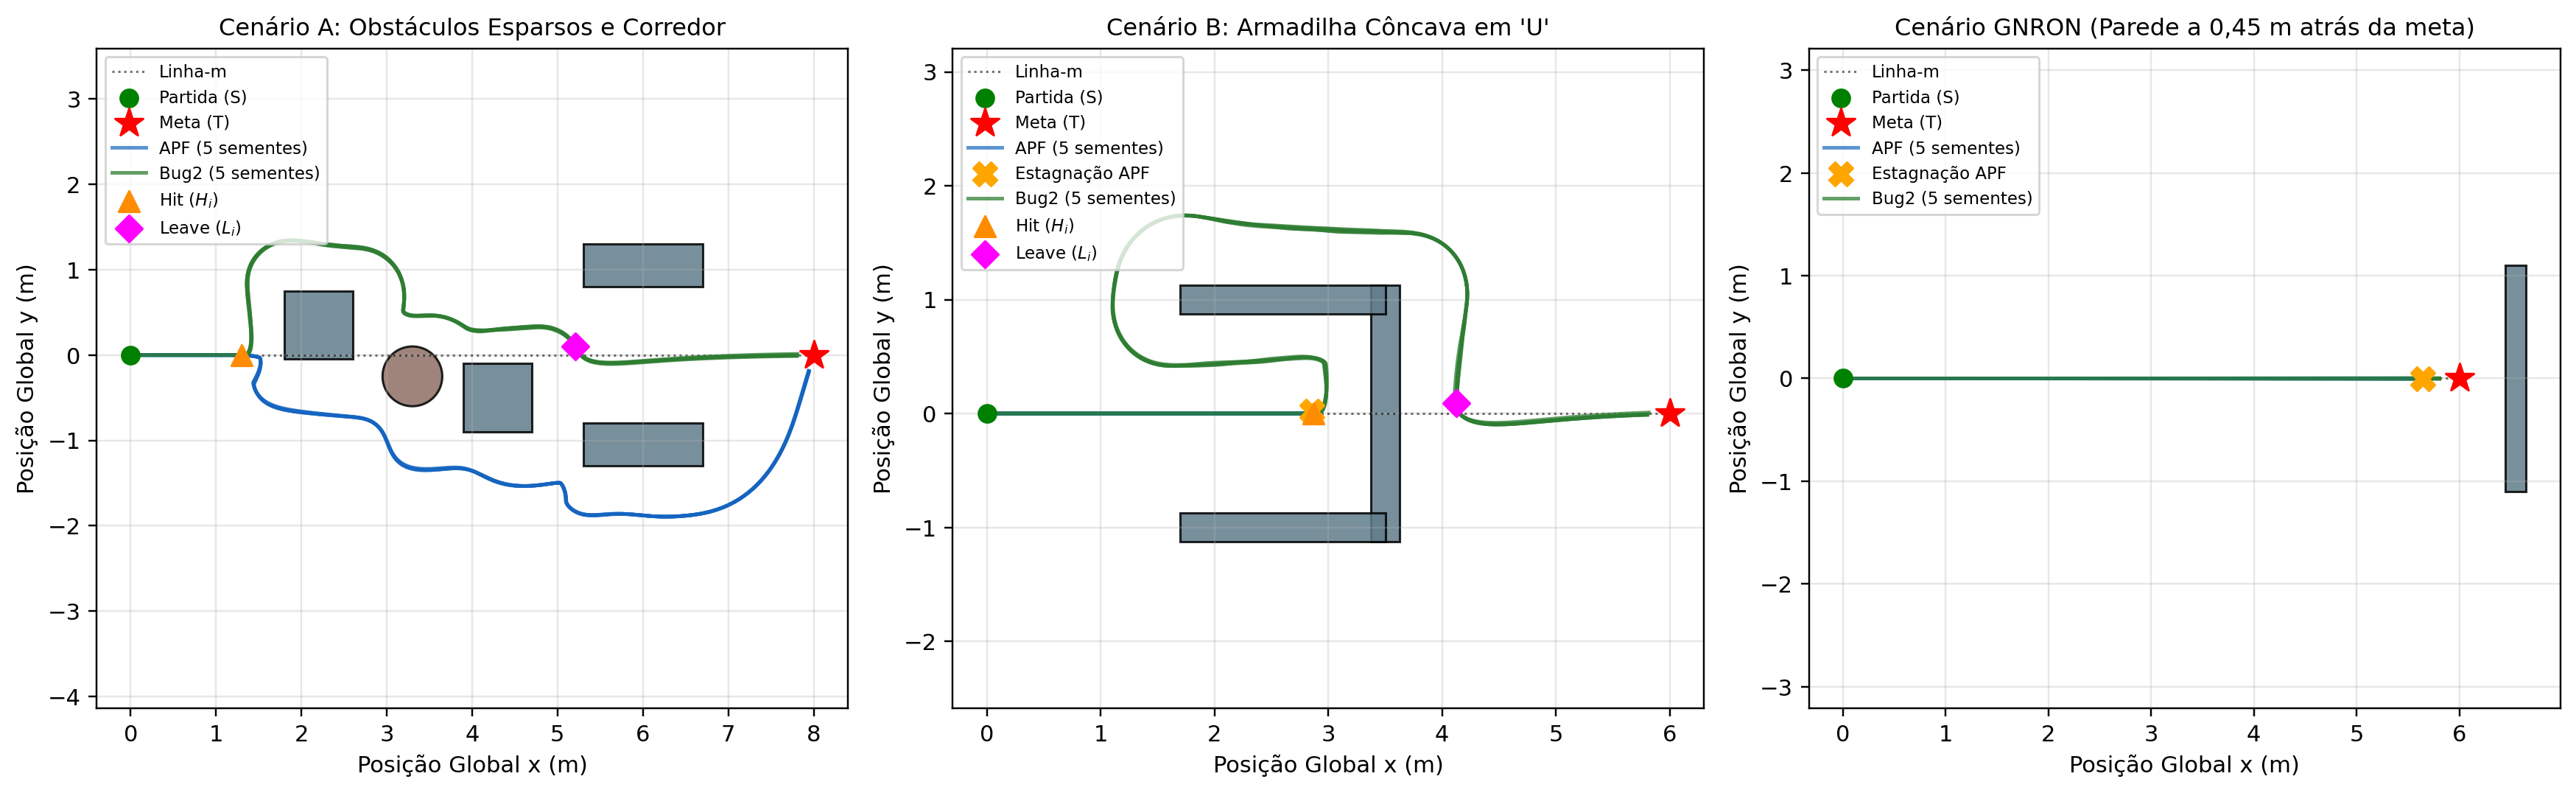
\includegraphics[width=\textwidth]{fig3_etapa2_comparacao_cenarios.png}
\caption{Trajetórias executadas (5 sementes) pelos métodos APF e Bug2 nos Cenários~A, B e no Subcenário GNRON.}
\label{fig:etapa2_cenarios}
\end{figure*}

\subsection{Estudo Paramétrico do APF e Limiar GNRON}
% TODO: Analisar a Figura~\ref{fig:etapa2_parametrico}:
% - Sensibilidade a (rho_0, k_rep) no Cenario A (colisoes na configuracao Fraco com d_min = 0,20 m vs. convergencia sem colisoes nas demais).
% - Efeito de rho_0 sobre o fenomeno GNRON (convergencia com rho_0 = 0,35 m < 0,45 m e estagnacao para rho_0 >= 0,80 m).

\begin{figure*}[t]
\centering
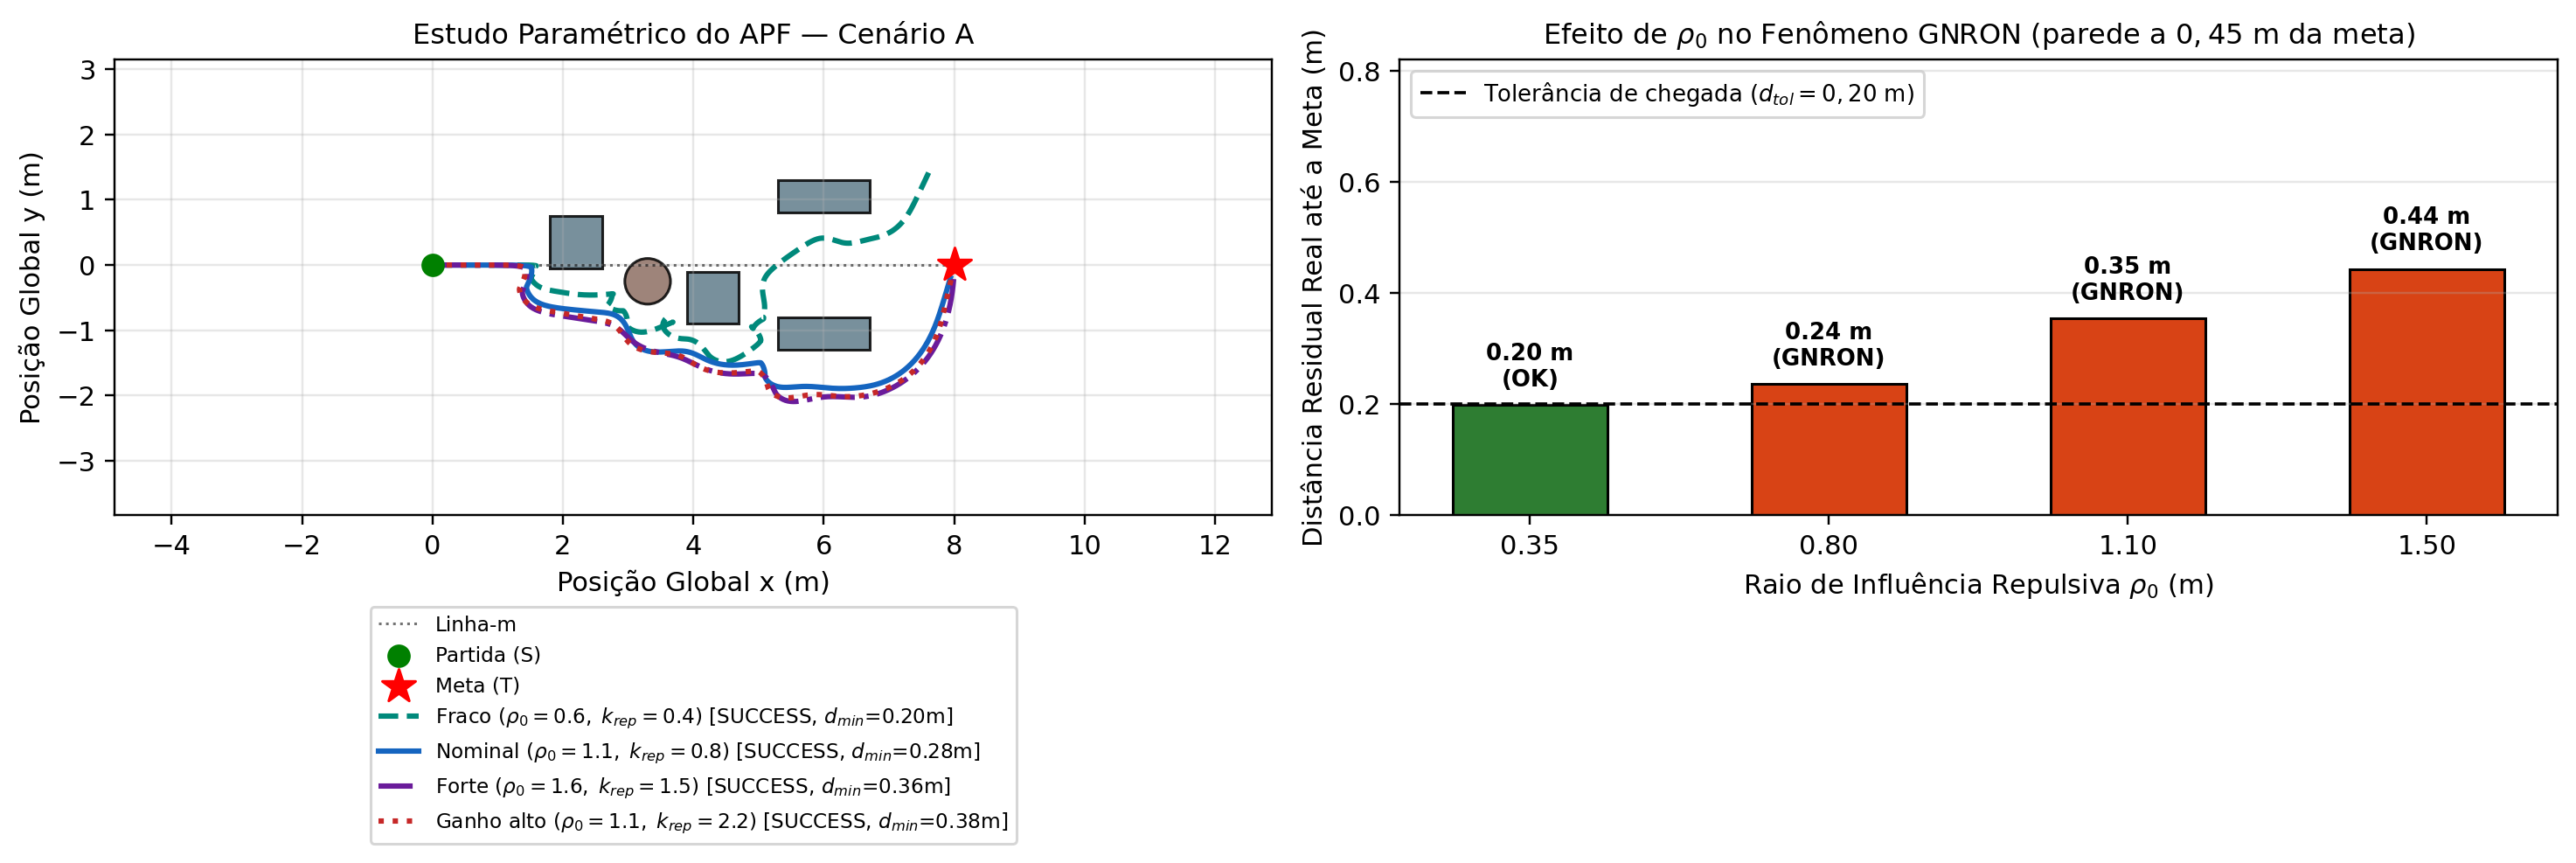
\includegraphics[width=\textwidth]{fig4_etapa2_estudo_parametrico.png}
\caption{Estudo paramétrico do APF no Cenário~A (esquerda) e efeito do raio de influência repulsiva $\rho_0$ no fenômeno GNRON (direita).}
\label{fig:etapa2_parametrico}
\end{figure*}

\section{Discussão Técnica e Limitações}

% TODO: Discutir criticamente os resultados observados:
% 1. Compromisso quantitativo entre APF (trajetorias mais suaves e rapidas em obstaculos esparsos) e Bug2 (garantia de convergencia em armadilhas concavas e maior margem d_min, ao custo de maior tempo/comprimento em contornos).
% 2. Interpretacao fisica/matematica da estagnacao do APF no Cenario B (anulacao F_att + F_rep = 0 em x ~ 2,85 m) e no Subcenario GNRON (relacao entre rho_0 e a distancia da parede atras da meta).
% 3. Influencia da odometria RK2 e do ruido sensorial (encoders e LiDAR) sobre a precisao final (e_p(t_f) < 1 cm nas execucoes sem colisao; degradacao acentuada em caso de colisao na configuracao Fraco).
% 4. Limitacoes da abordagem reativa classica (dependencia de estimativa odométrica sem correcao exteroceptiva em percursos longos, comportamento na linha-m sob deriva).

\section{Conclusões}

% TODO: Sintetizar:
% 1. Resposta direta a pergunta experimental do Projeto 6.
% 2. Principais resultados quantitativos da Etapa I (odometria RK2) e Etapa II (APF vs. Bug2 nos 3 cenarios e estudo parametrico).
% 3. Trabalhos futuros (fusao sensorial / localizacao global, extensao para navegacao embarcada em microcontroladores / TinyML com bancada Hardware-in-the-Loop).


\bibliographystyle{IEEEtran}
\bibliography{referencias}

\end{document}
